\subsection{Sección 5.4: Problema 12}

Muestre que si $f$ es continua en $[0,\infty)$ y uniformemente continua en $[a,\infty)$ para alguna constante positiva $a$, entonces $f$ es uniformemente continua en $[0,\infty)$. 
\begin{tcolorbox}[colback=blue!15,colframe=blue!1!blue,title=Definición de continuidad uniforme de \cite{bartle2000introduction}]
Sea $A\subseteq \mathbb{R}$ y sea $f: A\to\mathbb{R}$. Se dice que $f$ es uniformemente continua sobre $A$ si para cada $\epsilon>0$ existe un $\delta(\epsilon)>0$ tal que si $x,u\in A$ son cualesquiera números que satisfacen $|x-u|<\delta(\epsilon)$, entonces $|f(x)-f(u)|<\epsilon$.
\end{tcolorbox}
\begin{tcolorbox}[colback=gray!15,colframe=gray!1!gray,title= Teorema (Caracterización de la compacidad en $\mathbf{R}$) de \cite{abbott2012understanding} ]
Un conjunto $K\subseteq\mathbf{R}$ es compacto si y solo si es cerrado y acotado. 
\end{tcolorbox}

\begin{tcolorbox}[colback=gray!15,colframe=gray!1!gray,title= Teorema  (Heine-Borel) de \cite{abbott2012understanding} ]
Sea $K$ un subconjunto de $\mathbf{R}$. Todos los enunciados siguientes son equivalentes en el sentido que cualquier de ellos, implica los otros dos. 
\begin{enumerate}
    \item $K$ es compacto. 
    \item $K$ es cerrado y acotado.
    \item Cada cubierta abierta para $K$ tiene una subconvierta finita. 
\end{enumerate}
\end{tcolorbox}

\begin{tcolorbox}[colback=gray!15,colframe=gray!1!gray,title= Teorema (Continuidad uniforme en conjuntos compactos) de \cite{abbott2012understanding}]
Una función que es continua en un conjnto compacto $K$ es uniformemente continua en $K$. 

\end{tcolorbox}

\begin{proof}
Por hipótesis tenemos que $f$ es continua en $[0,\infty)$ y es uniformemente continua en $[a,\infty)$ para alguna constante positiva $a$. A probar: $f$ es uniformemente continua en $[0,\infty)$. Es decir: 

\begin{center}
    

\tikzset{every picture/.style={line width=0.75pt}} %set default line width to 0.75pt        

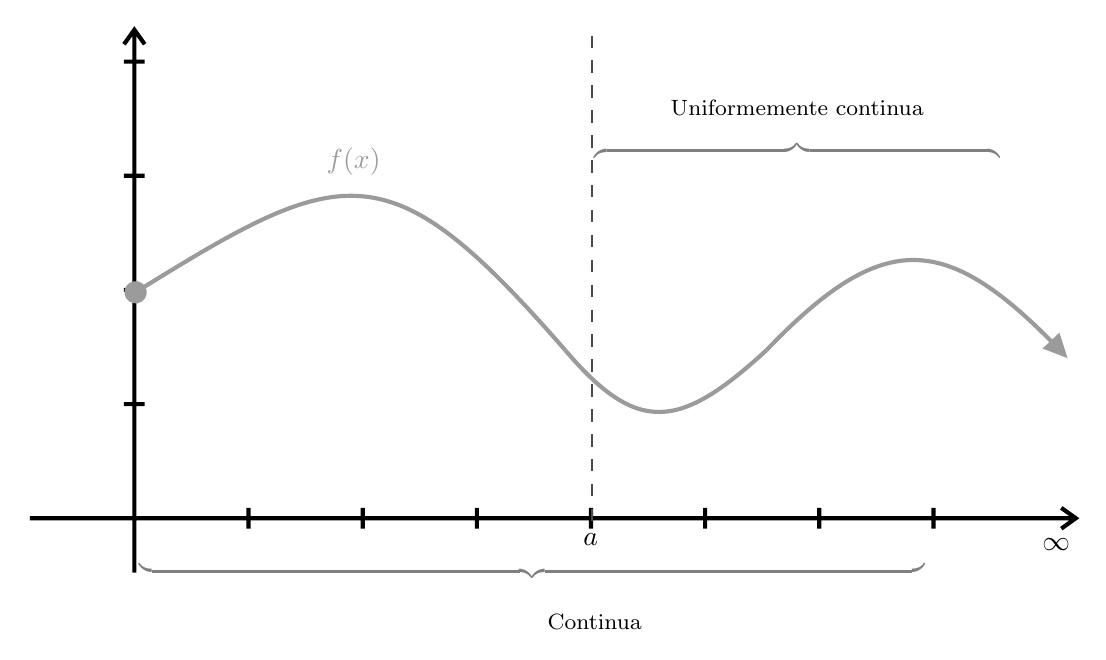
\begin{tikzpicture}[x=0.75pt,y=0.75pt,yscale=-1,xscale=1]
%uncomment if require: \path (0,300); %set diagram left start at 0, and has height of 300

%Shape: Axis 2D [id:dp4838826961855275] 
\draw [color={rgb, 255:red, 0; green, 0; blue, 0 }  ,draw opacity=1 ][line width=1.5]  (79.43,240.99) -- (583.43,240.99)(129.83,5.64) -- (129.83,267.14) (576.43,235.99) -- (583.43,240.99) -- (576.43,245.99) (124.83,12.64) -- (129.83,5.64) -- (134.83,12.64) (184.83,235.99) -- (184.83,245.99)(239.83,235.99) -- (239.83,245.99)(294.83,235.99) -- (294.83,245.99)(349.83,235.99) -- (349.83,245.99)(404.83,235.99) -- (404.83,245.99)(459.83,235.99) -- (459.83,245.99)(514.83,235.99) -- (514.83,245.99)(124.83,185.99) -- (134.83,185.99)(124.83,130.99) -- (134.83,130.99)(124.83,75.99) -- (134.83,75.99)(124.83,20.99) -- (134.83,20.99) ;
\draw   ;
%Curve Lines [id:da8876476568884512] 
\draw [color={rgb, 255:red, 155; green, 155; blue, 155 }  ,draw opacity=1 ][line width=1.5]    (130.43,132.14) .. controls (231.43,69.22) and (252.36,62.41) .. (337.51,160.12) ;
\draw [shift={(130.43,132.14)}, rotate = 328.08] [color={rgb, 255:red, 155; green, 155; blue, 155 }  ,draw opacity=1 ][fill={rgb, 255:red, 155; green, 155; blue, 155 }  ,fill opacity=1 ][line width=1.5]      (0, 0) circle [x radius= 4.36, y radius= 4.36]   ;
%Curve Lines [id:da029640962564212336] 
\draw [color={rgb, 255:red, 155; green, 155; blue, 155 }  ,draw opacity=1 ][line width=1.5]    (434.28,160.12) .. controls (491.47,100.54) and (521.43,103.26) .. (576.88,161.16) ;
\draw [shift={(579.43,163.85)}, rotate = 226.65] [fill={rgb, 255:red, 155; green, 155; blue, 155 }  ,fill opacity=1 ][line width=0.08]  [draw opacity=0] (11.61,-5.58) -- (0,0) -- (11.61,5.58) -- cycle    ;
%Curve Lines [id:da6106144459124002] 
\draw [color={rgb, 255:red, 155; green, 155; blue, 155 }  ,draw opacity=1 ][line width=1.5]    (337.51,160.12) .. controls (372.35,201.07) and (392.67,198.28) .. (434.28,160.12) ;
%Straight Lines [id:da22950199783318004] 
\draw [color={rgb, 255:red, 74; green, 74; blue, 74 }  ,draw opacity=1 ] [dash pattern={on 4.5pt off 4.5pt}]  (350.13,8.43) -- (350.13,243.88) ;

% Text Node
\draw (344.67,246.66) node [anchor=north west][inner sep=0.75pt]    {$a$};
% Text Node
\draw (552.53,249.45) node [anchor=north west][inner sep=0.75pt]    {$\ \ \ \infty $};
% Text Node
\draw (349.89,57.54) node [anchor=north west][inner sep=0.75pt]  [color={rgb, 255:red, 128; green, 128; blue, 128 }  ,opacity=1 ]  {$\overbrace{\ \ \ \ \ \ \ \ \ \ \ \ \ \ \ \ \ \ \ \ \ \ \ \ \ \ \ \ \ \ \ \ \ \ \ \ \ \ \ \ \ \ \ \ }$};
% Text Node
\draw (386.71,37.92) node [anchor=north west][inner sep=0.75pt]  [font=\footnotesize] [align=left] {Uniformemente continua};
% Text Node
\draw (131,260.21) node [anchor=north west][inner sep=0.75pt]  [font=\small,color={rgb, 255:red, 128; green, 128; blue, 128 }  ,opacity=1 ]  {$\underbrace{\ \ \ \ \ \ \ \ \ \ \ \ \ \ \ \ \ \ \ \ \ \ \ \ \ \ \ \ \ \ \ \ \ \ \ \ \ \ \ \ \ \ \ \ \ \ \ \ \ \ \ \ \ \ \ \ \ \ \ \ \ \ \ \ \ \ \ \ \ \ \ \ \ \ \ \ \ \ \ \ \ \ \ \ \ \ \ \ \ \ \ \ }$};
% Text Node
\draw (301,285.79) node [anchor=north west][inner sep=0.75pt]  [font=\footnotesize] [align=left] { \ \ \ \ \ \ \ Continua};
% Text Node
\draw (221,61.21) node [anchor=north west][inner sep=0.75pt]  [color={rgb, 255:red, 155; green, 155; blue, 155 }  ,opacity=1 ]  {$f( x)$};


\end{tikzpicture}
\end{center}

Nótese que lo que nos piden es demostrar que el intervalo $[0,a]$ es uniformemente continuo y posteriormente demostrar que $[0,\infty)$ es continuo. 

\linita 

$\implies$ Sabemos que $[0,a]$ es acotado y cerrado. $\implies$ Por Heine-Borel y la caracterización de la compacidad en $\mathbb{R}$, $[0,a]$ es compacto. $\implies$ Por el teorema de la continuidad uniforme en conjuntos compactos, $[0,a]$ es uniformemente continua.  $\implies$ Para evitar lidiar con las situaciones que pueden darse alrededor de $a$, se preferirá trabajar con una de los cotas, es decir: $[0,a+1]$, que también es uniformemente continua. 

\linita 

Ahora, es necesario probar que $[0,\infty)$ es uniformemente continua. Procederemos con la definición de continuidad para los dos subconjuntos $[0,a+1]$ y $[a,\infty)$.

\linita 

\begin{noter}{Notación}
$$\delta_1(\epsilon)=\delta_1 \quad \text{ y }\quad  \delta_2(\epsilon)=\delta_2$$
\end{noter}
$\implies$ Dado $\epsilon>0$, existe un $0<\delta_1<1$ tales que $x,u\in [0,a+1]$ son cualesquiera números que satisfacen $|x-u|<\delta_1$, entonces $|f(x)-f(u)|<\epsilon$. Además, existe un $0<\delta_2<1$ tales que $x,u\in[0,\infty)$ son cualesquiera números que satisfacen $|x-u|<\delta_2$, entonces $|f(x)-f(u)|<\epsilon$. Ahora bien, elijamos arbitrariamente que $\delta:= \min\{\delta_1,\delta_2\}$ tal que exista $\delta<1$ tales que $x,u\in[0,a+1]$ o $x,u\in[a,\infty)$ son cualesquiera números que satisfacen $|x-u|<\delta$, entonces: 

$$|f(x)-f(u)|<\epsilon.$$

Por lo tanto, $f$ es uniformemente continua.
\end{proof}